\section{Bug Reporting in Open Source Projects}


%The problem is real, i.e., there are repos that have more BRs than they can manage. How many BRs arrive at the most popular repos (is the traffic bursty)? how many lack OB/EB/S2R from these?
The overall trend in software development in recent years is towards increased
speed of development and delivery. There are nowadays numerous projects on popular
public software collaboration platforms like GitHub that have large development
teams and user communities. Many of these projects experience significant
bug reporting traffic~\cite{Zhang2014ASO}. Figure~\ref{fig:repo_activity} shows the issue creation
frequency for a selection of ten GitHub repositories that are currently active
with a high numbers of commits and developers. Three of these repositories have
a median of over 40 issues created daily, where most of them are bug reports reported by
GitHub identities that have not contributed to the project (i.e., users). In addition,
the same three projects exhibit high variance in daily issue creation, likely indicative
of bursty and hard to predict bug reporting activity. This is a
considerable burden for bug triagers and it motivates the need for the type of work
as described in this paper, which intends to make bug triage more efficient and less of
a burden for project maintainers.

\begin{figure}[t]
\centering
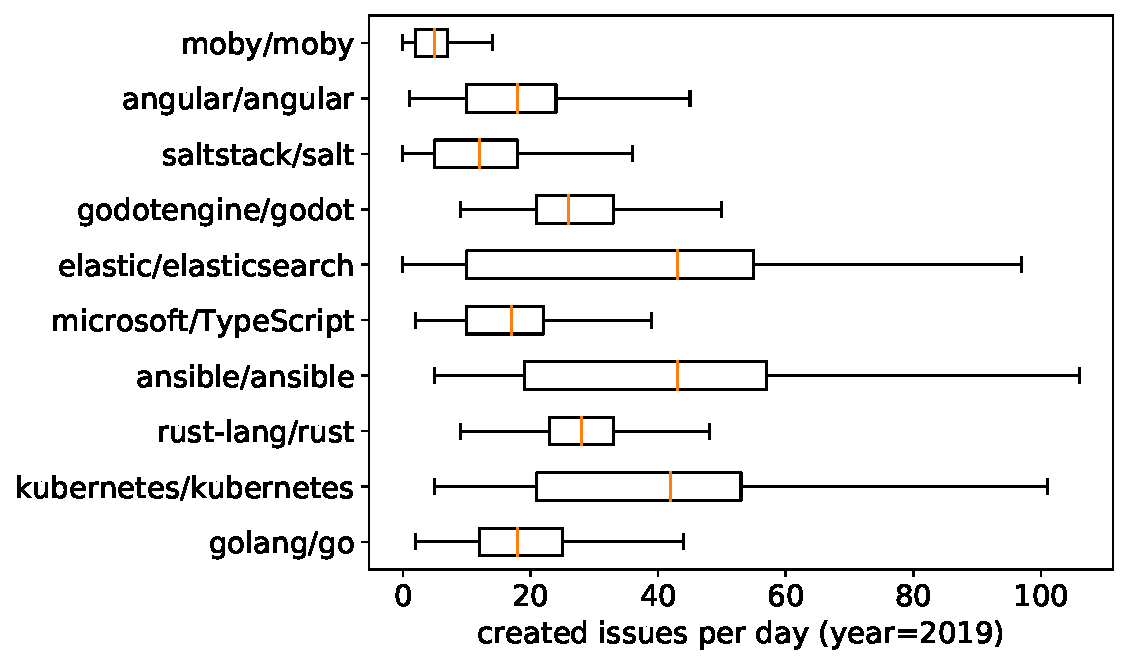
\includegraphics[width=0.99\linewidth]{figures/popular_repos.pdf}
\caption{Daily issue creation activity in 2019 for a selection of ten highly active
(by number of commits) repositories on GitHub.}
\label{fig:repo_activity}
\end{figure}


\begin{table}[t]
\centering
\caption{Evaluation results contrasting our system (\evpi) relative to several baselines.}
\begin{tabular}{p{3cm}cccc}
\hline
%                          & \multicolumn{4}{c}{$V_{1} \cap V_{2}$} \\\hline
                          & {\bf MRR}  & {\bf P@1}  & {\bf P@3}  & {\bf P@5}  \\\hline
{\em Random}              & 0.52 & 0.32 & 0.33 & 0.34 \\
{\em Lucene}              & 0.53 & 0.35 & 0.32 & 0.32 \\
{\em Utility only}        & 0.65 & 0.47 & 0.44 & 0.41 \\
{\em Compatibility only}  & 0.61 & 0.43 & 0.38 & 0.38 \\
{\em \evpi}                & 0.67 & 0.49 & 0.49 & 0.45 \\ \hline
\end{tabular}
\label{tab:results}
\end{table}



% The preconditions are present, i.e., there are a lot of follow-up questions on GitHub -- we could
% use the same set of 10 repos to show this.
Posing follow-up questions is an already practiced mitigation strategy for deficient bug
reports. To lend support for this claim and to quantify how wide spread is the use of
follow-up questions, we performed a small scale study of the prevalence
of follow-up questions on GitHub, focusing on the 10 active projects used in Figure~\ref{fig:repo_activity}.
We randomly sampled 50 closed bug reports for each of the 10 repositories (500 in total) and manually examined them
for follow-up questions. We were also interested whether the answers to those questions (if they are present) provide any
of the three key parts of a bug report: Observable Behavior, Expected Behavior or Steps to Reproduce.
Table~\ref{tab:sample} shows that...




The availability of existing follow-up questions on social coding platforms like GitHub provides the
preconditions for the approach described in this paper, which leverages such existing follow-up questions
to automatically rank and select the most appropriate of them for a newly written, incomplete bug report.



Motivate EB, OB and S2R as a way of ranking by a follow-up question.
{\em Agnieszka: cite What makes a good bug report - developers value S2R as the most helpful, OB is 4th.}